\chapter{\ifproject%
\ifenglish Experimentation and Results\else การทดลองและผลลัพธ์\fi
\else%
\ifenglish System Evaluation\else การประเมินระบบ\fi
\fi}

% ในบทนี้จะทดสอบเกี่ยวกับการทำงานในฟังก์ชันหลักๆ
ในบทนี้จะทดสอบระบบการยืนยันตัวตนด้วยการใช้ภาพใบหน้าบุคคล ซึ่งมีการเก็บข้อมูลรูปภาพใบหน้าบุคคล เพื่อทำการทดลองเป็นเวลา 5 วัน แล้วดูผลการทดลองในแต่ละวัน ได้แก่ 
ความแม่นยำในการตรวจจับรูปภาพใบหน้าบุคคล ความแม่นยำของการระบุตัวตนด้วยรูปภาพใบหน้าบุคคล เวลาในการประมวลผลรูปภาพใบหน้าบุคคลตลอดถึงการแสดงผล 
และความพึงพอใจของผู้ทดลองต่อระบบ


\section{ความแม่นยำของการตรวจจับใบหน้า}
การทดสอบนี้จะเป็นการทดสอบเพื่อวัดผลความแม่นยำในการตรวจจับภาพใบหน้าบุคคล โดยมีรูปภาพใบหน้าบุคคลจำนวน 50 รูป และรูปภาพสัตว์จำนวน 50 รูป 
ทำการทดลองกับแบบจำลองการตรวจจับใบหน้าบุคคลได้ผลลัพธ์ดังกราฟด้านล่าง

\begin{figure}[!ht]
  \begin{center}
    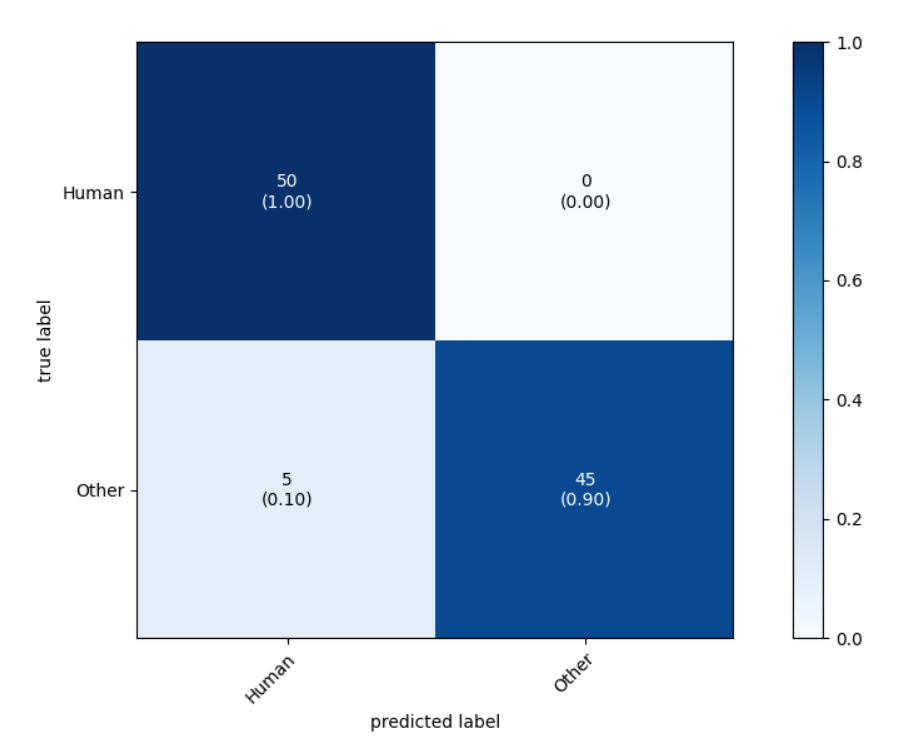
\includegraphics[scale=.45]{pic/face_result.png}
    \caption[กราฟแสดงความแม่นยำของการตรวจจับใบหน้า]{กราฟแสดงความแม่นยำของการตรวจจับใบหน้า}
    \label{fig:acc_graph}
  \end{center}
\end{figure}

\indent จากกราฟจะสามารถคำนวนความแม่นยำได้ดังสูตร 
\begin{equation}\label{eq:Precision}
Precision=\frac{True Positive}{True Positive + False Positive}=\frac{50}{50+0} = 1.0
\end{equation}

\begin{equation}\label{eq:Accuracy}
Accuracy=\frac{True Positive + True Nagative}{Positive + Negative}=\frac{50+45}{50+50} = 0.95
\end{equation}

\begin{equation}\label{eq:F1Score}
F1 Score=\frac{2\cdot True Positive}{2\cdot True Positive + False Positive + False Negative}=\frac{2\cdot 50}{2\cdot 50+0+5} = 0.9524
\end{equation}

\section{ความแม่นยำของการระบุตัวตนด้วยใบหน้าในแต่ละวัน}
การทดสอบนี้จะเป็นการทดสอบเพื่อวัดผลความแม่นยำในการระบุตัวตน โดยความแม่นยำจะมีแนวโน้มที่เพิ่มขึ้นหรือลดลงตามจำนวนวันที่ตรวจจับภาพใบหน้าบุคคล
เนื่องจากใช้กลวิธีการเรียนรู้ของเครื่องแบบต่อเนื่อง ซึ่งการทดลองนี้จะบันทึกผลลัพธ์การระบุตัวตนในทุกครั้งที่มีการตรวจจับภาพใบหน้าบุคคลไว้ที่เซิร์ฟเวอร์และ Raspberry Pi 
ในรูปแบบของ JSON และส่งผลลัพธ์การระบุตัวตนกลับไปยังมอดูลกล้องเพื่อแสดงผลลัพธ์การระบุตัวตนให้ผู้ใช้งานได้ทราบ 
โดยรูปที่ \ref*{fig:face_graph} จะแสดงกราฟผลลัพธ์ความแม่นยำของการระบุตัวตนหนึ่งคนจากผู้ทดลองทั้งหมด 
โดยจะนำข้อมูลที่ได้บันทึกจากทั้งสองแหล่งมาเปรียบเทียบความผิดพลาดของข้อมูลการระบุตัวตน

\begin{figure}[!ht]
    \begin{center}
      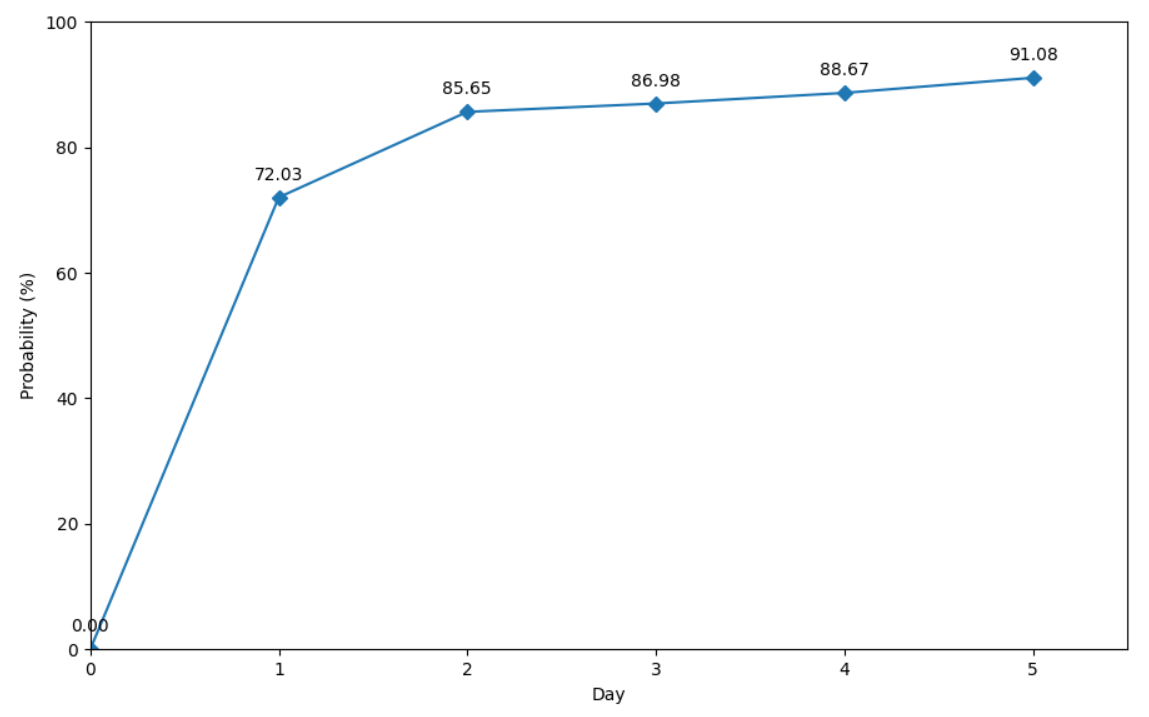
\includegraphics[scale=.5]{pic/Note_percent.png}
      \caption[กราฟแสดงความแม่นยำของการระบุตัวตนในแต่ละวัน]{กราฟแสดงความแม่นยำของการระบุตัวตนในแต่ละวัน}
      \label{fig:face_graph}
    \end{center}
  \end{figure}

\indent จากกราฟจะเห็นว่าความแม่นยำของการระบุตัวตนในวันที่ 1 คือ 73.03 เปอร์เซ็นต์ และในวันที่ 5 คือ 91.08 เปอร์เซ็นต์ ซึ่งเป็นไปตามหลักการเรียนรู้ของเครื่องแบบต่อเนื่อง


\section{เวลาในการประมวลผลรูปภาพใบหน้า}
การทดสอบต่อไปนี้เป็นการทดสอบเพื่อวัดผลเวลาทั้งหมดของการประมวลผลรูปภาพใบหน้า ส่งรูปภาพไปยังเซิร์ฟเวอร์ ระบุตัวตน และการส่งผลลัพธ์กลับมาแสดงผลในหน้าจอ
โดยจะวัดเวลาในหน่วยของมิลลิวินาที (Millisecond) และบันทึกผลที่ Raspberry Pi โดยจะเปรียบเทียบเวลาที่วัดได้ในทุกครั้งที่มีการตรวจจับภาพใบหน้า 
ซึ่งจำนวนครั้งที่ตรวจจับใบหน้าบุคคลคือ 207 ครั้งจากทั้งหมด 5 วันที่ทำการทดลองแล้วสรุปผลออกมาเป็นกราฟ
  
\begin{figure}[!ht]
  \begin{center}
    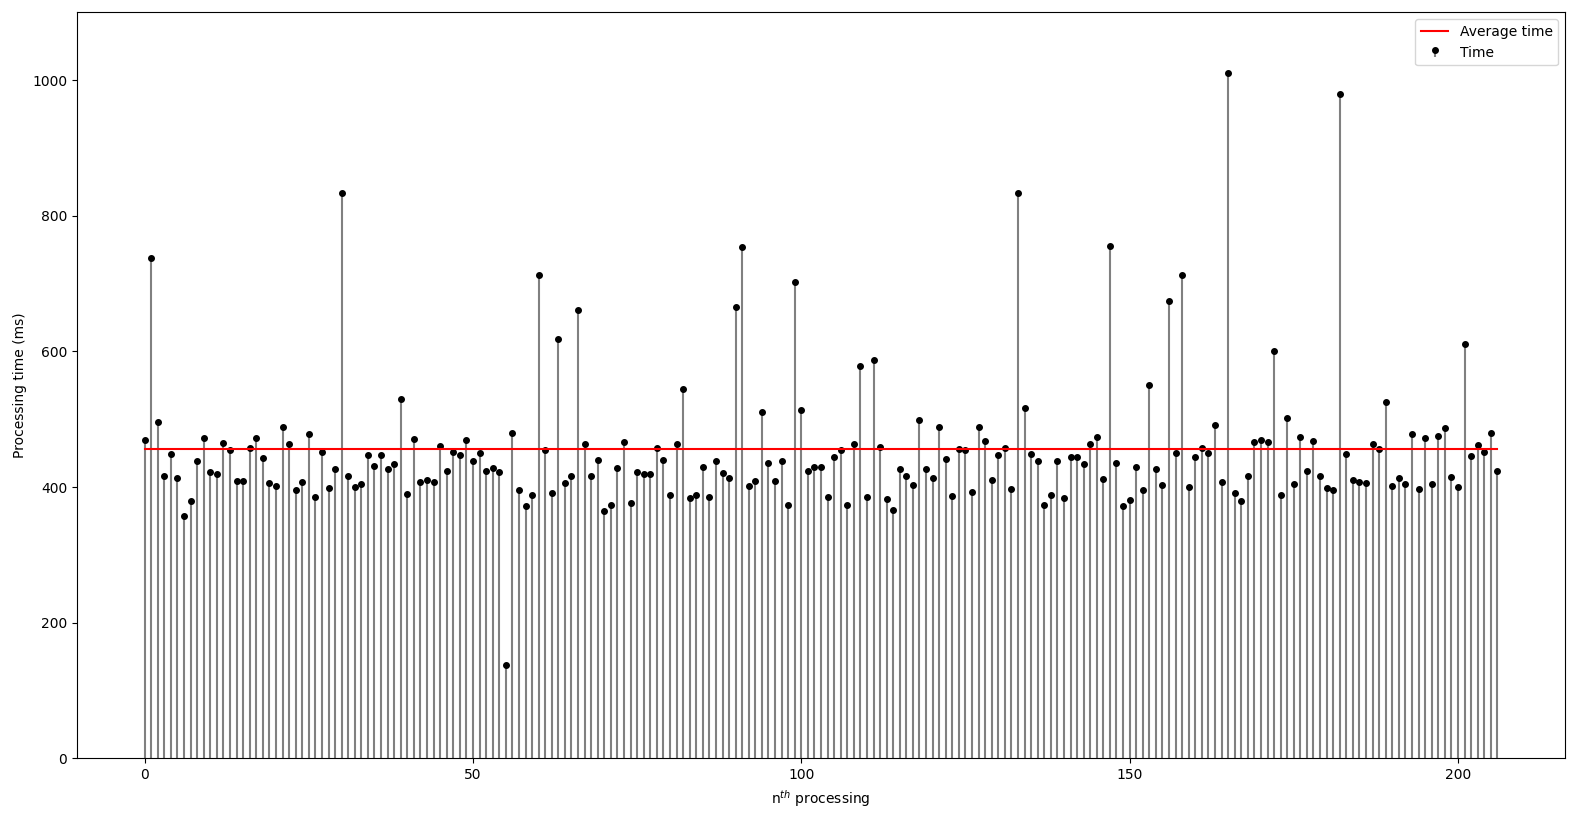
\includegraphics[scale=.5]{pic/Time_1.png}
    \caption[กราฟแสดงเวลาในการประมวลผลของระบบในแต่ละวัน]{กราฟแสดงเวลาในการประมวลผลของระบบในแต่ละวัน}
    \label{fig:time_graph}
  \end{center}
\end{figure}
\newpage
\indent จากกราฟจะเห็นได้ว่าเวลาในการประมวลผลรูปภาพใบหน้า ส่งรูปภาพไปยังเซิร์ฟเวอร์ การระบุตัวตน และการส่งผลลัพธ์กลับมาแสดงผลในหน้าจอนั้นมีเวลาเฉลี่ย 455.618 มิลลิวินาที



\section{ความพึงพอใจของการทดลอง}
จากการทดลองที่ห้องวิจัย OASYS ได้ทำการบันทึกผลความพึงพอใจของผู้ทดลองต่อระบบระบุตัวตนด้วยรูปภาพใบหน้าบุคคลที่ โดยจะได้ผลสรุปดังนี้

\begin{figure}[!ht]
    \begin{center}
      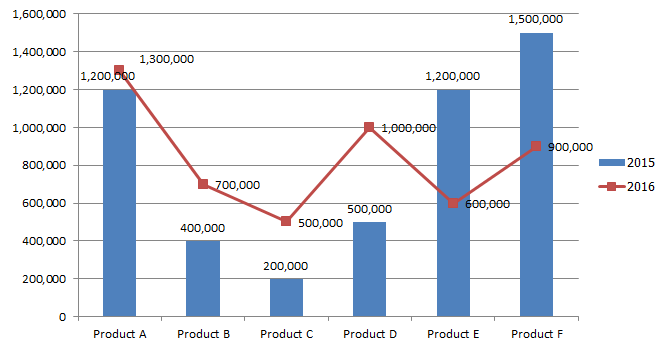
\includegraphics[scale=.5]{pic/bar_graph.png}
      \caption[กราฟแสดงความพึงพอใจของผู้ทดลอง]{กราฟแสดงความพึงพอใจของผู้ทดลอง}
      \label{fig:bar_graph}
    \end{center}
  \end{figure}